\chapter{Bylgjuhreyfing í fleti}
Þegar bylgja breiðir úr getur færst út í allar áttir, í fyrri köflum
hefur bara verið skoðað tilfellið þegar bylgja breiðist út
í einni vídd. Núna er hægt að taka fyrir þegar bylgja breiðist
út tveim víddum, s.s. fleti. Þá er hægt lýsa nokkrum gerðum af
bylgjuútbreiðslum, sem hringjum og línum.

\section{Bylgjustafn}
Bylgjustafn er þegar við táknum með línu hvar bylgjutoppur er
í fletinum. S.s meðfram línunni er toppurinn á bylgju sem er að breiðast
út, á meðan tíminn líður mun línan ferðast áfram og hugsanlega breyta
lögun.

Bylgjustafnar geta verkað saman eða á móti hvor öðrum, það er hægt að
hafa til dæmis 2 bylgjustafna sem verka með eða gegn hvor öðrum. Þá
er samliðun líka gild fyrir bylgjur í fleti jafnt til bylgna í einni
vídd. Þá geta bylgjustafnar komið í mörgum formum, hér verður einungis
tekið fyrir kúlubylgjur og línubylgjur.

Kúlurbylgjur byrja í punkti og dreifast síðan jafnt í allar, tíðni
bylgjustafnsins myndi þá vera háð fjölda skipta á sekúndu sem
punkturinn myndar nýjan bylgjustafn. Eftirfarandi mynd sýnir
tvær tímamyndir, þar sem $b_1$ táknar fyrsta bylgjustafn og
$b_2$ táknar annan bylgjustafn, $b_3$ þriðja, o.s.f. Þannig
er hægt að sýna staðsetningu stafnsins
\begin{center}
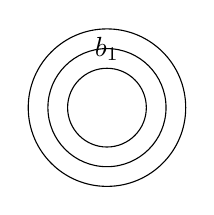
\begin{tikzpicture}
	\draw[color = black] (0,0) circle(0.50);
	\draw[color = black] (0,0) circle(0.75) +(0,0.75) node {$b_1$};
	\draw[color = black] (0,0) circle(1.00);
\end{tikzpicture}
\end{center} 

Þá myndast nýr stafn í hvert sinn, hinsvegar þegar tími líður ferðast
stafninn áfram og er hraði bylgjunar kallaður bylgjuhraði eða
oftar útbreiðsluhraði bylgjunar, s.s. hversu hratt bylgjan breiðir
úr sér. Mælieiningin sem er er notuð er mæld í metrum per sekúndu eða
$\uspeedms$.

Þegar bylgjustafn er bein lína er hægt að ímynda sér sett af línum
sem myndast og ferðast síðan fram á við
\begin{center}
\begin{tikzpicture}
	\draw[color = black] (0,0) -- (0,1) node[above] {$b_1$};
\end{tikzpicture}
\end{center}

\subsection{Bylgjustafn og brot}
Þegar flatur bylgjustafn lendir á littlu gati getur hann umbreyst frá því
að vera flatur stafn yfir í að verða kúlustafn. Í raun er stafninn ennþá
,,flatur'' í fyrri skilgreiningi, bara í stað þess að vilja fara beint
áfram er það styttra að ferðast meðfram bogaferli en að þvinga sig beint
áfram. Ef opið er haft nægilega breitt þá myndast beinn stafn að hluta
til en ef opið er of lítið getur enginn stafn myndast.
\begin{center}
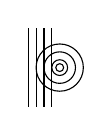
\begin{tikzpicture}
	\draw[color = black] (0,0) -- (0,1);
	\draw[color = black] (0.1,0) -- (0.1,1);
	\draw[color = black] (0.2,0) -- (0.2,1);
	\draw[color = black] (0.3,0) -- (0.3,1);
	\draw[color = black] (0.4,0.5) circle(0.05);
	\draw[color = black] (0.4,0.5) circle(0.1);
	\draw[color = black] (0.4,0.5) circle(0.2);
	\draw[color = black] (0.4,0.5) circle(0.3);
\end{tikzpicture}
\end{center}
til að prufa slíkt í raunveruleikanum er kjörið að prufa slíkt með vatni
í bala. Með því að dýfa littlum pinna í vatnið er hægt að skapa
kúlustafn og með því að dýfa þunnum ferköntuðum hlut í vatn er hægt að
skapa flatbylgjur.

\section{Lögmál Huygens}
Hægt er að nýta lögmál Huygens til að finna bylgjustafn frá við mismunandi
punktbrot og línubrotl.

\section{Ljósbognun}

\section{Samliðun í föstum efnum}
Bylgjur sem ferðast í gegnum efni geta náð að mynda samliðun með reglulegu
millibili. Þá er hægt að ímynda sér að bylgjustafn sem lendir þvert á
sett af atómum og myndar kúlubylgju í stað fyrir þverbylgju. Frá hverju
atómi kemur kúlubylgja sem myndar gagnlega og eyðandi samliðun við hin
atómin. Sem stærð er hægt að setja það í jöfnuform á hvaða hornum
samliðunum á sér stað. Gagnleg samliðun gerist við
\begin{align}
	\unumbern \uwavelength_\unumbern &= \ulengthd \sin{ \varphi_\unumbern } 
\end{align}
fyrir eyðandi samliðun þá er jafan
\begin{align}
	\frac{\unumbern}{2} \uwavelength_\unumbern &= \ulengthd \sin{ \phi_\unumbern } 
\end{align}
sönnunin á þessu er áhugaverð blanda af hornafræði og bylgjuútbreiðslu.
Fyrir gagnlega samliðun þá er bara hægt að tala um algjöra samliðun þegar
bylgjutopparnir eru eina bylgjulengd frá hvor öðrum.
\\
\begin{center}
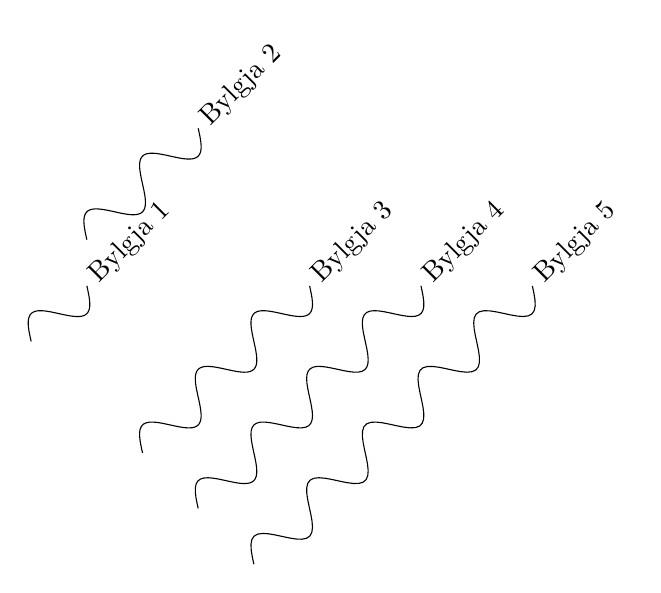
\begin{tikzpicture}[
	force/.style={>=latex,draw=blue,fill=blue, very thick},
	forcecomp/.style={>=latex,draw=blue, densely dashed, fill=blue},
	axis/.style={densely dashed,gray,font=\small},
	m/.style={rectangle,draw=black,fill=gray,minimum size=0.3cm,thin},
	M/.style={rectangle,draw,fill=lightgray,minimum size=0.3cm,thin},
	scale=1,
	domain=0:{3.141*2}
	]
	\draw[color = black, samples=100, domain=0:{3.141*2*1}, rotate=45] 
		plot({\x/3.141/2},{0.25*sin(\x r)}) node[right, rotate=45] {Bylgja 1};
	\draw[color = black, samples=100, domain=0:{3.141*2*2}, yshift=2cm, rotate=45] 
		{plot(\x/3.141/2,{0.25*sin(\x r)-1.0})} node[right, rotate=45] {Bylgja 2};
	\draw[color = black, samples=100, domain=0:{3.141*2*3}, rotate=45] 
		plot(\x/3.141/2,{0.25*sin(\x r)-2.0}) node[right, rotate=45] {Bylgja 3};
	\draw[color = black, samples=100, domain=0:{3.141*2*4}, rotate=45] 
		plot(\x/3.141/2,{0.25*sin(\x r)-3.0}) node[right, rotate=45] {Bylgja 4};
	\draw[color = black, samples=100, domain=0:{3.141*2*5}, rotate=45] 
		plot(\x/3.141/2,{0.25*sin(\x r)-4.0}) node[right, rotate=45] {Bylgja 5};
\end{tikzpicture}
\end{center}

\section{Lögmál Braggs}
% add thin diffraction
Þegar bylgjustafn (oft röntgen geislar) lendir á atómum myndast gagnleg samliðun sem er eins og 
hefðbundin samliðun, nema hvað það kemur auka tala með sem tvölfaldar
bylgjulengdina á stafninum. Úr því kemur lögmál Braggs sem er einungis hægt
að nota fyrir þunnar himnur.
\begin{equation}
	\unumbern \uwavelength_\unumbern = 2\ulengthd \sin{ \varphi_\unumbern }
\end{equation}
til að sanna þetta lögmál er hægt að búa til teikningu sem sýnir hvaðan
þessi tvöföldun kemur \\
\begin{center}
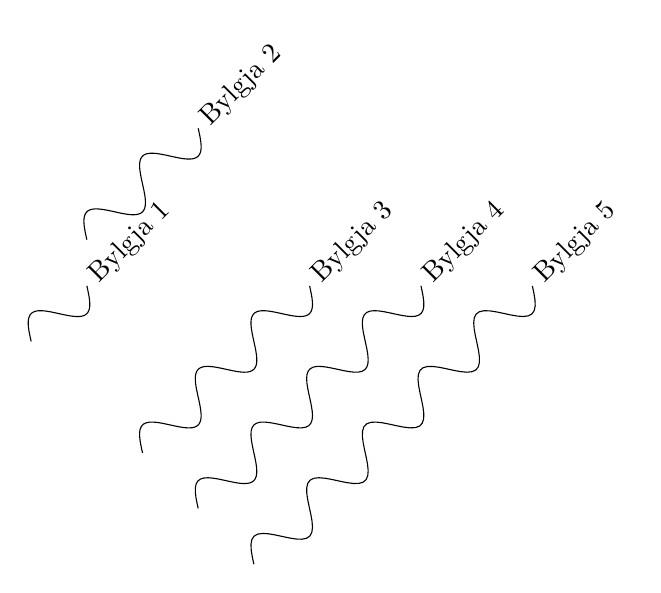
\begin{tikzpicture}[
	force/.style={>=latex,draw=blue,fill=blue, very thick},
	forcecomp/.style={>=latex,draw=blue, densely dashed, fill=blue},
	axis/.style={densely dashed,gray,font=\small},
	m/.style={rectangle,draw=black,fill=gray,minimum size=0.3cm,thin},
	M/.style={rectangle,draw,fill=lightgray,minimum size=0.3cm,thin},
	scale=1,
	domain=0:{3.141*2}
	]
	\draw[color = black, samples=100, domain=0:{3.141*2*1}, rotate=45] 
		plot({\x/3.141/2},{0.25*sin(\x r)}) node[right, rotate=45] {Bylgja 1};
	\draw[color = black, samples=100, domain=0:{3.141*2*2}, yshift=2cm, rotate=45] 
		{plot(\x/3.141/2,{0.25*sin(\x r)-1.0})} node[right, rotate=45] {Bylgja 2};
	\draw[color = black, samples=100, domain=0:{3.141*2*3}, rotate=45] 
		plot(\x/3.141/2,{0.25*sin(\x r)-2.0}) node[right, rotate=45] {Bylgja 3};
	\draw[color = black, samples=100, domain=0:{3.141*2*4}, rotate=45] 
		plot(\x/3.141/2,{0.25*sin(\x r)-3.0}) node[right, rotate=45] {Bylgja 4};
	\draw[color = black, samples=100, domain=0:{3.141*2*5}, rotate=45] 
		plot(\x/3.141/2,{0.25*sin(\x r)-4.0}) node[right, rotate=45] {Bylgja 5};
\end{tikzpicture}
\end{center}

